% --- IMPORTS ---
\documentclass[leqno]{article}
\usepackage{graphicx}
\usepackage{dsfont}
\usepackage{mathtools}
\usepackage{amssymb}
\usepackage{amsmath}
\usepackage{amsthm}
\usepackage{float}
\usepackage{ragged2e}
\usepackage{tensor}
\usepackage{fancyhdr}
\usepackage{empheq}
\usepackage[most]{tcolorbox}
\usepackage{enumitem}
\usepackage{dirtytalk}
\usepackage{marginnote}
\usepackage{microtype}
\usepackage[
  a4paper,
  left=0.8in,
  right=1in,
  top=1in,
  bottom=0.5in,
  headheight=14pt,
  headsep=0.4in
]{geometry}
\setlength{\parindent}{0cm}
% --- TikZ Packages ---
\usepackage{pgfplots}
\pgfplotsset{compat=1.18}
\usepgfplotslibrary{fillbetween, polar}
\usetikzlibrary{calc, positioning}
\usetikzlibrary{angles, quotes}
\usetikzlibrary{arrows.meta}
\usetikzlibrary{decorations.pathreplacing, decorations.markings}
\usetikzlibrary{patterns}
\usetikzlibrary{intersections}
% --- URL Packages ---
\usepackage[colorlinks=true,linkcolor=red,citecolor=magenta,urlcolor=black]{hyperref}%
\urlstyle{same}
% --- END OF IMPORTS ---

% --- CUSTOM COMMANDS ---
\RenewDocumentCommand{\marks}{o m}{%
  \IfValueTF{#1}%
    {\marginnote{\raggedright\textbf{[#2]}}[#1]}%
    {\marginnote{\raggedright\textbf{[#2]}}}%
}
\newcommand{\vspacerule}[2]{%
  \par\vspace*{#1}%
  \noindent\hrulefill\par
  \vspace*{#2}%
}
\definecolor{scarlet}{RGB}{205, 40, 75}
\newcommand{\questionitem}{%
  \item\phantomsection
  \addcontentsline{toc}{section}{Question \number\value{enumi}}%
}
\renewcommand{\contentsname}{Questions}
% --- END OF CUSTOM COMMANDS ---

% --- HEADER CONFIG ---
\pagestyle{fancy}
\fancyhead{}
\fancyfoot{}
\renewcommand{\headrulewidth}{0.9pt}
\lhead{\textit{Solutions} - Hyperbolic Functions}
\chead{}
\rhead{\href{https://danieljsmith.org}{danieljsmith.org}}
% --- END OF HEADER CONFIG ---

\begin{document}
\vspace*{20pt}
\tableofcontents
\newpage
\begin{enumerate}[
  label=\textbf{\arabic*.},
  leftmargin=*,
  topsep=0pt,
  partopsep=0pt,
  parsep=0pt
]

% ---- Question 1 ----
\questionitem

The curve $C_1$ has equation \[y=2\cosh 2x-2\] and the curve $C_2$ has equation \[y=3-5e^{-2x}\] \\
\begin{enumerate}[label=\textbf{(\alph*)}]
  \item Sketch the graphs of $C_1$ and $C_2$ on one set of axes, giving the equation of any asymptote and the coordinates of the points where the curves meet the axes. \marks{4} \\
  \item Solve the equation $2\cosh 2x-2=3-5e^{-2x}$, giving your answers in the form $\frac{1}{2}\ln k$, where $k$ is an integer. \marks{5} \\
\end{enumerate}

\vspace*{10pt}

\begin{tcolorbox}[colback=white, colframe=scarlet, title={\textbf{Solution}}, breakable, grow to left by=6mm, grow to right by=10mm]
\begin{enumerate}[label=\textbf{(\alph*)}]
  \item The sketch should look like:

\begin{tikzpicture}
\begin{axis}[
    axis lines=middle,
    xmin=-1.2, xmax=1.2,
    ymin=-5, ymax=9.5,
    width=0.78\linewidth,
    height=10cm,
    samples=300,
    clip=false,
    xlabel style={at={(rel axis cs:1,0)}, anchor=west},
    ylabel style={at={(rel axis cs:0,1)}, anchor=south},
    xtick={0},
    ytick={-2},
    tick label style={font=\small},
    label style={font=\small},
    every axis plot/.append style={thick}
]
\addplot[domain=-1.2:1.2] {exp(2*x)+exp(-2*x)-2};
\addplot[domain=-0.23:1.2] {3-5*exp(-2*x)};
\addplot[dashed, domain=-1.2:1.18, samples=2] {3};
\node[fill=white, inner sep=1pt] at (axis cs:0.93,5.9) {$C_1$};
\node[fill=white, inner sep=1pt] at (axis cs:0.90,1.7) {$C_2$};
\node[fill=white, inner sep=1pt] at (axis cs:-0.3,3.45) {$y=3$};
\end{axis}
\end{tikzpicture}

$C_1$ is the graph of $y=\cosh x$ scaled horizontally and vertically. Like $y=\cosh x $ it meets the coordinate axes at the origin $(0, 0)$ only, and has no asymptotes. \\

$C_2$ is the graph of $y=3-5e^{-2x}$. As $x\rightarrow \infty,\, e^{-2x}\rightarrow0$ so $y\rightarrow3$. Thus $C_2$ has a horizontal asymptote at $y=3.$

$C_2$ meets the $y$-axis when $x=0$: $y = 3-5e^{-2(0)} = 3 - 5 =-2$. So the y-intercept is $(0, -2)$.

$C_2$ meets the $x$-axis when $3-5e^{-2x}=0$. Solving this equation obtains $x=\frac{1}{2}\ln\frac{5}{3}$, so the $x$-intercept is \[\left(\frac{1}{2}\ln\frac{5}{3}, 0\right)\] 


  \item Solve
\[
2\cosh 2x-2=3-5e^{-2x}
\]
Using
\[
2\cosh 2x=e^{2x}+e^{-2x}
\]
gives
\[
e^{2x}+e^{-2x}-2=3-5e^{-2x}
\]
so
\[
e^{2x}+e^{-2x}=5-5e^{-2x}
\]

Let
\[
t=e^{2x}
\]
Then \(t>0\) and \(e^{-2x}=\dfrac1t\). Substituting,
\[
t+\frac1t=5-\frac5t
\]
Multiplying through by \(t\),
\[
t^2+1=5t-5
\]
\[
t^2-5t+6=0
\]
\[
(t-2)(t-3)=0
\]
Hence
\[
t=2 \quad \text{or} \quad t=3
\]

Since \(t=e^{2x}\),
\[
e^{2x}=2 \quad \text{or} \quad e^{2x}=3
\]
Taking logarithms,
\[
2x=\ln 2 \quad \text{or} \quad 2x=\ln 3
\]
Therefore
\[
x=\frac12\ln 2 \quad \text{or} \quad x=\frac12\ln 3
\]

So the solutions are \(x=\frac12\ln 2\) and \(x=\frac12\ln 3\).
\end{enumerate}
\end{tcolorbox}


\newpage

% ---- Question 2 ----
\questionitem

\begin{enumerate}[label=\textbf{(\alph*)}]
  \item Use the definitions of $\sinh x$ and $\cosh x$ in terms of exponentials to show that
  \[
  \tanh x \equiv \frac{e^{2x}-1}{e^{2x}+1}
  \]
  \marks[-20pt]{2}
  \item Hence find the value of $x$ for which
  \[
  \tanh(x-\ln 2)=\frac{3}{7}
  \]
  giving your answer in the form $\dfrac{1}{2}\ln k$, where $k$ is a rational number to be determined. \marks{5} \\
\end{enumerate}

\vspace*{10pt}

\begin{tcolorbox}[colback=white, colframe=scarlet, title={\textbf{Solution}}, breakable, grow to left by=6mm, grow to right by=10mm]
\begin{enumerate}[label=\textbf{(\alph*)}]
  \item Using the definitions
  \[
  \sinh x=\frac{e^x-e^{-x}}{2}
  \qquad \text{and} \qquad
  \cosh x=\frac{e^x+e^{-x}}{2}
  \]
  we have
  \begin{align*}
  \tanh x
  &=\frac{\sinh x}{\cosh x} \\
  &=\frac{\frac{e^x-e^{-x}}{2}}{\frac{e^x+e^{-x}}{2}} \\
  &=\frac{e^x-e^{-x}}{e^x+e^{-x}}
  \end{align*}
  Now multiply numerator and denominator by $e^x$:
  \begin{align*}
  \tanh x
  &=\frac{(e^x-e^{-x})e^x}{(e^x+e^{-x})e^x} \\
  &=\frac{e^{2x}-1}{e^{2x}+1}
  \end{align*}
  Hence
  \[
  \tanh x \equiv \frac{e^{2x}-1}{e^{2x}+1}
  \]

  \item Let
  \[
  y=x-\ln 2
  \]
  Then the equation becomes
  \[
  \tanh y=\frac{3}{7}
  \]
  Using the result from part (a),
  \[
  \frac{e^{2y}-1}{e^{2y}+1}=\frac{3}{7}
  \]
  Cross-multiplying:
  \begin{align*}
  7(e^{2y}-1)&=3(e^{2y}+1) \\
  7e^{2y}-7&=3e^{2y}+3 \\
  4e^{2y}&=10 \\
  e^{2y}&=\frac{5}{2}
  \end{align*}
  Taking natural logarithms:
  \begin{align*}
  2y&=\ln\!\left(\frac{5}{2}\right)
  \end{align*}
  Since $y=x-\ln 2$,
  \begin{align*}
  2(x-\ln 2)&=\ln\!\left(\frac{5}{2}\right) \\
  2x-2\ln 2&=\ln\!\left(\frac{5}{2}\right)
  \end{align*}
  So
  \begin{align*}
  2x
  &=\ln\!\left(\frac{5}{2}\right)+2\ln 2 \\
  &=\ln\!\left(\frac{5}{2}\right)+\ln 4 \\
  &=\ln\!\left(\frac{5}{2}\times 4\right) \\
  &=\ln 10
  \end{align*}
  Therefore
  \[
  x=\frac{1}{2}\ln 10
  \]
\end{enumerate}
\end{tcolorbox}


\newpage

% ---- Question 3 ----
\questionitem

\begin{enumerate}[label=\textbf{(\alph*)}]
  \item Express $7\cosh x - 5\sinh x$ in the form $R\cosh(x - \alpha)$, where $R > 0$ and $\alpha > 0$.\\ Give $\alpha$ to $3$ decimal places. \marks{4} \\
  \item Hence solve the equation $7\cosh x - 5\sinh x = 10$, giving all solutions correct to $2$ decimal places. \marks{3} \\
  \item Solve $7\cosh x - 5\sinh x = 10$ by instead using the exponential definitions of $\cosh x$ and $\sinh x$. \marks{4} \\
\end{enumerate}

\vspace*{10pt}

\begin{tcolorbox}[colback=white, colframe=scarlet, title={\textbf{Solution}}, breakable, grow to left by=6mm, grow to right by=10mm]
\begin{enumerate}[label=\textbf{(\alph*)}]
  \item Using
  \[
  \cosh(x-\alpha)=\cosh x\cosh\alpha-\sinh x\sinh\alpha
  \]
  we have
  \[
  R\cosh(x-\alpha)=R\cosh x\cosh\alpha-R\sinh x\sinh\alpha
  \]
  
  Comparing this with
  \[
  7\cosh x-5\sinh x
  \]
  gives
  \[
  R\cosh\alpha=7,
  \qquad
  R\sinh\alpha=5
  \]
  
  Now use \(\cosh^2\alpha-\sinh^2\alpha=1\):
  \begin{align*}
  R^2(\cosh^2\alpha-\sinh^2\alpha)&=7^2-5^2\\
  R^2&=49-25\\
  R^2&=24
  \end{align*}
  Since \(R>0\),
  \[
  R=2\sqrt6
  \]
  
  Also,
  \[
  \tanh\alpha=\frac{\sinh\alpha}{\cosh\alpha}=\frac{5/R}{7/R}=\frac57
  \]
  so
  \begin{align*}
  \alpha&=\operatorname{artanh}\left(\frac57\right)\\
  &=\frac12\ln\left(\frac{1+\frac57}{1-\frac57}\right)\\
  &=\frac12\ln 6
  \end{align*}
  Hence
  \[
  \alpha\approx 0.896
  \]
  
  Therefore
  \[
  7\cosh x-5\sinh x=2\sqrt6\cosh\left(x-\tfrac12\ln6\right)
  \]
  with
  \[
  R=2\sqrt6,
  \qquad
  \alpha=\frac12\ln6\approx 0.896
  \]

  \item From part (a),
  \[
  7\cosh x-5\sinh x=2\sqrt6\cosh\left(x-\tfrac12\ln6\right)
  \]
  so the equation becomes
  \[
  2\sqrt6\cosh\left(x-\tfrac12\ln6\right)=10
  \]
  Hence
  \[
  \cosh\left(x-\tfrac12\ln6\right)=\frac{5}{\sqrt6}
  \]
  
  Therefore
  \[
  x-\tfrac12\ln6=\pm \operatorname{arcosh}\left(\frac{5}{\sqrt6}\right)
  \]
  so
  \[
  x=\tfrac12\ln6\pm \operatorname{arcosh}\left(\frac{5}{\sqrt6}\right)
  \]
  
  Using
  \[
  \operatorname{arcosh}u=\ln\left(u+\sqrt{u^2-1}\right)
  \]
  gives
  \begin{align*}
  \operatorname{arcosh}\left(\frac{5}{\sqrt6}\right)
  &=\ln\left(\frac{5}{\sqrt6}+\sqrt{\frac{25}{6}-1}\right)\\
  &=\ln\left(\frac{5}{\sqrt6}+\sqrt{\frac{19}{6}}\right)\\
  &=\ln\left(\frac{5+\sqrt{19}}{\sqrt6}\right)
  \end{align*}
  
  So
  \begin{align*}
  x&=\ln(\sqrt6)\pm \ln\left(\frac{5+\sqrt{19}}{\sqrt6}\right)\\
  &=\ln(5+\sqrt{19})
  \quad \text{or} \quad
  \ln\left(\frac{6}{5+\sqrt{19}}\right)
  \end{align*}
  Rationalising,
  \[
  \frac{6}{5+\sqrt{19}}=5-\sqrt{19}
  \]
  so
  \[
  x=\ln(5+\sqrt{19})
  \quad \text{or} \quad
  x=\ln(5-\sqrt{19})
  \]
  
  Therefore the solutions are
  \[
  x\approx 2.24 \quad \text{or} \quad x\approx -0.44
  \]

  \item Using the definitions
  \[
  \cosh x=\frac{e^x+e^{-x}}{2},
  \qquad
  \sinh x=\frac{e^x-e^{-x}}{2}
  \]
  the equation
  \[
  7\cosh x-5\sinh x=10
  \]
  becomes
  \begin{align*}
  7\left(\frac{e^x+e^{-x}}{2}\right)-5\left(\frac{e^x-e^{-x}}{2}\right)&=10\\
  \frac{7e^x+7e^{-x}-5e^x+5e^{-x}}{2}&=10\\
  \frac{2e^x+12e^{-x}}{2}&=10\\
  e^x+6e^{-x}&=10
  \end{align*}
  
  Multiply through by \(e^x\):
  \[
  e^{2x}-10e^x+6=0
  \]
  
  Let \(y=e^x\), so \(y>0\). Then
  \[
  y^2-10y+6=0
  \]
  Solving the quadratic,
  \begin{align*}
  y&=\frac{10\pm\sqrt{100-24}}{2}\\
  &=\frac{10\pm\sqrt{76}}{2}\\
  &=5\pm\sqrt{19}
  \end{align*}
  
  Since both values are positive,
  \[
  e^x=5+\sqrt{19}
  \quad \text{or} \quad
  e^x=5-\sqrt{19}
  \]
  Hence
  \[
  x=\ln(5+\sqrt{19})
  \quad \text{or} \quad
  x=\ln(5-\sqrt{19})
  \]
  
  Therefore
  \[
  x\approx 2.24 \quad \text{or} \quad x\approx -0.44
  \]
\end{enumerate}
\end{tcolorbox}


\newpage

% ---- Question 4 ----
\questionitem

\begin{enumerate}[label=\textbf{(\alph*)}]
  \item Starting from the identity $\cosh 2x = 2\cosh^2 x - 1$, prove that
  \[
  \operatorname{sech} 2x = \frac{\operatorname{sech}^2 x}{2-\operatorname{sech}^2 x}
  \]
  \marks[-30pt]{2}
  \item The function $f$ is defined by
  \[
  f(x)=\operatorname{sech} x \qquad (x>0)
  \]
  \begin{enumerate}[label=(\roman*)]
    \item State the range of $f$. \marks{1}
    \item Use part (a) and part (b)(i) to prove that $\operatorname{sech} 2x<\operatorname{sech} x$ if $x>0$. \marks{3} \\
  \end{enumerate}
\end{enumerate}

\vspace*{10pt}

\begin{tcolorbox}[colback=white, colframe=scarlet, title={\textbf{Solution}}, breakable, grow to left by=6mm, grow to right by=10mm]
\begin{enumerate}[label=\textbf{(\alph*)}]
  \item Starting with
  \[
  \cosh 2x = 2\cosh^2 x - 1
  \]
  take reciprocals:
  \[
  \operatorname{sech} 2x=\frac{1}{\cosh 2x}=\frac{1}{2\cosh^2 x-1}
  \]
  Now use \(\operatorname{sech} x=\dfrac{1}{\cosh x}\), so that
  \[
  \cosh^2 x=\frac{1}{\operatorname{sech}^2 x}
  \]
  Hence
  \begin{align*}
  \operatorname{sech} 2x
  &=\frac{1}{2\left(\dfrac{1}{\operatorname{sech}^2 x}\right)-1} \\
  &=\frac{1}{\dfrac{2-\operatorname{sech}^2 x}{\operatorname{sech}^2 x}} \\
  &=\frac{\operatorname{sech}^2 x}{2-\operatorname{sech}^2 x}
  \end{align*}
  So
  \[
  \operatorname{sech} 2x = \frac{\operatorname{sech}^2 x}{2 - \operatorname{sech}^2 x}
  \]

  \item
  \begin{enumerate}[label=(\roman*)]
    \item For \(x>0\), we have \(\cosh x>1\), so
    \[
    0<\operatorname{sech} x=\frac{1}{\cosh x}<1
    \]
    Also, as \(x\to 0^+\), \(\operatorname{sech} x\to 1\), and as \(x\to \infty\), \(\operatorname{sech} x\to 0\).

    Therefore the range of \(f\) is
    \[
    (0,1)
    \]

    \item Let
    \[
    t=\operatorname{sech} x
    \]
    From part (b)(i), since \(x>0\),
    \[
    0<t<1
    \]
    Using part (a),
    \[
    \operatorname{sech} 2x=\frac{t^2}{2-t^2}
    \]
    Since \(0<t<1\), we have \(0<t^2<1\), so
    \[
    2-t^2>1
    \]
    Therefore
    \[
    \frac{t^2}{2-t^2}<t^2
    \]
    and because \(0<t<1\),
    \[
    t^2<t
    \]
    Hence
    \[
    \operatorname{sech} 2x=\frac{t^2}{2-t^2}<t=\operatorname{sech} x
    \]
    So, for \(x>0\),
    \[
    \operatorname{sech} 2x<\operatorname{sech} x
    \]
  \end{enumerate}
\end{enumerate}
\end{tcolorbox}


\newpage

% ---- Question 5 ----
\questionitem

By writing $\sinh x$ and $\cosh x$ in terms of exponentials, solve the equation \[2\sinh x+5\cosh x=6\] giving your solutions in exact logarithmic form. \marks{6}

\vspace*{10pt}

\begin{tcolorbox}[colback=white, colframe=scarlet, title={\textbf{Solution}}, breakable, grow to left by=6mm, grow to right by=10mm]
Write the hyperbolic functions in exponential form:
\[
\sinh x=\frac{e^x-e^{-x}}{2},
\qquad
\cosh x=\frac{e^x+e^{-x}}{2}
\]

Substitute these into the equation \(2\sinh x+5\cosh x=6\):
\begin{align*}
2\left(\frac{e^x-e^{-x}}{2}\right)+5\left(\frac{e^x+e^{-x}}{2}\right)&=6\\
e^x-e^{-x}+\frac{5}{2}e^x+\frac{5}{2}e^{-x}&=6\\
\frac{7}{2}e^x+\frac{3}{2}e^{-x}&=6
\end{align*}

Multiply through by \(2e^x\):
\begin{align*}
2e^x\left(\frac{7}{2}e^x+\frac{3}{2}e^{-x}\right)&=2e^x\cdot 6\\
7e^{2x}+3&=12e^x
\end{align*}

So
\[
7e^{2x}-12e^x+3=0
\]

Let
\[
y=e^x
\]
Then \(y>0\), and the equation becomes
\[
7y^2-12y+3=0
\]

Solve this quadratic:
\begin{align*}
y&=\frac{12\pm\sqrt{(-12)^2-4\cdot 7\cdot 3}}{2\cdot 7}\\
&=\frac{12\pm\sqrt{144-84}}{14}\\
&=\frac{12\pm\sqrt{60}}{14}\\
&=\frac{12\pm 2\sqrt{15}}{14}\\
&=\frac{6\pm\sqrt{15}}{7}
\end{align*}

Hence
\[
e^x=\frac{6+\sqrt{15}}{7}
\quad \text{or} \quad
e^x=\frac{6-\sqrt{15}}{7}
\]

Both values are positive, so both are valid. Taking natural logarithms gives
\[
x=\ln\left(\frac{6+\sqrt{15}}{7}\right)
\quad \text{or} \quad
x=\ln\left(\frac{6-\sqrt{15}}{7}\right)
\]

Therefore the exact solutions are
\[
x=\ln\left(\frac{6+\sqrt{15}}{7}\right)
\quad \text{and} \quad
x=\ln\left(\frac{6-\sqrt{15}}{7}\right)
\]
\end{tcolorbox}


\newpage

% ---- Question 6 ----
\questionitem

\begin{enumerate}[label=\textbf{(\alph*)}]
  \item Using the definitions of $\sinh x$ and $\cosh x$ in terms of exponentials, show that \[\cosh 2x = 1+2\sinh^2 x\] \marks[-20pt]{2} 
  \item Hence solve the equation \[2\cosh 2x-7\sinh x=4\] giving all your answers in logarithmic form. \marks{5} \\
\end{enumerate}

\vspace*{10pt}

\begin{tcolorbox}[colback=white, colframe=scarlet, title={\textbf{Solution}}, breakable, grow to left by=6mm, grow to right by=10mm]
\begin{enumerate}[label=\textbf{(\alph*)}]
  \item Using
\[
\sinh x=\frac{e^x-e^{-x}}{2}
\qquad \text{and} \qquad
\cosh x=\frac{e^x+e^{-x}}{2}
\]
we have
\begin{align*}
\cosh 2x
&=\frac{e^{2x}+e^{-2x}}{2} \\
&=1+\frac{e^{2x}-2+e^{-2x}}{2} \\
&=1+\frac{(e^x-e^{-x})^2}{2} \\
&=1+2\left(\frac{e^x-e^{-x}}{2}\right)^2 \\
&=1+2\sinh^2 x
\end{align*}
So
\[
\cosh 2x=1+2\sinh^2 x
\]

  \item Using the result from part (a),
\begin{align*}
2\cosh 2x-7\sinh x&=4 \\
2(1+2\sinh^2 x)-7\sinh x&=4
\end{align*}
Let \(s=\sinh x\). Then
\begin{align*}
2+4s^2-7s&=4 \\
4s^2-7s-2&=0 \\
(4s+1)(s-2)&=0
\end{align*}
So
\[
\sinh x=2 \qquad \text{or} \qquad \sinh x=-\frac14
\]

First, if \(\sinh x=2\), then
\begin{align*}
\frac{e^x-e^{-x}}{2}&=2 \\
e^x-e^{-x}&=4
\end{align*}
Multiplying by \(e^x\),
\begin{align*}
e^{2x}-1&=4e^x \\
e^{2x}-4e^x-1&=0
\end{align*}
Let \(y=e^x\), where \(y>0\). Then
\[
y^2-4y-1=0
\]
so
\[
y=\frac{4\pm\sqrt{16+4}}{2}=2\pm\sqrt5
\]
Since \(y>0\), we take \(y=2+\sqrt5\). Hence
\[
x=\ln(2+\sqrt5)
\]

Second, if \(\sinh x=-\frac14\), then
\begin{align*}
\frac{e^x-e^{-x}}{2}&=-\frac14 \\
e^x-e^{-x}&=-\frac12
\end{align*}
Multiplying by \(2e^x\),
\begin{align*}
2e^{2x}-2&=-e^x \\
2e^{2x}+e^x-2&=0
\end{align*}
Let \(y=e^x\), where \(y>0\). Then
\[
2y^2+y-2=0
\]
so
\[
y=\frac{-1\pm\sqrt{1+16}}{4}=\frac{-1\pm\sqrt{17}}{4}
\]
Since \(y>0\), we take
\[
y=\frac{\sqrt{17}-1}{4}
\]
Hence
\[
x=\ln\!\left(\frac{\sqrt{17}-1}{4}\right)
\]

Therefore the solutions are
\[
x=\ln(2+\sqrt5)
\qquad \text{or} \qquad
x=\ln\!\left(\frac{\sqrt{17}-1}{4}\right)
\]
\end{enumerate}
\end{tcolorbox}


\newpage

% ---- Question 7 ----
\questionitem

\begin{enumerate}[label=\textbf{(\alph*)}]
  \item Prove that, for $x\ge 1$,
  \[
  \operatorname{arcosh} x = \ln\left(x+\sqrt{x^2-1}\right)
  \]
  \marks[-20pt]{5}
  \item Prove that the graphs of
  \[
  y=\operatorname{arsinh} x \quad \text{and} \quad y=\operatorname{arcosh}(x+2)
  \]
  do not intersect. \marks{3} \\
\end{enumerate}

\vspace*{10pt}

\begin{tcolorbox}[colback=white, colframe=scarlet, title={\textbf{Solution}}, breakable, grow to left by=6mm, grow to right by=10mm]
\begin{enumerate}[label=\textbf{(\alph*)}]
  \item Let
\[
y=\operatorname{arcosh}x
\]
Then, by definition of the inverse hyperbolic cosine, \(y\geq 0\) and
\[
x=\cosh y=\frac{e^y+e^{-y}}{2}
\]
Now let
\[
t=e^y
\]
Since \(e^y>0\), we have \(t>0\), and also \(e^{-y}=\dfrac1t\). So
\[
2x=t+\frac1t
\]
Multiplying by \(t\),
\[
2xt=t^2+1
\]
so
\[
t^2-2xt+1=0
\]
This is a quadratic in \(t\), so
\begin{align*}
t&=\frac{2x\pm\sqrt{(2x)^2-4}}{2}\\
&=\frac{2x\pm\sqrt{4x^2-4}}{2}\\
&=x\pm\sqrt{x^2-1}
\end{align*}
Hence
\[
e^y=x\pm\sqrt{x^2-1}
\]

We now choose the correct sign. Since \(y\geq 0\),
\[
e^y\geq 1
\]
Also,
\begin{align*}
x-\sqrt{x^2-1}
&=\frac{(x-\sqrt{x^2-1})(x+\sqrt{x^2-1})}{x+\sqrt{x^2-1}}\\
&=\frac{x^2-(x^2-1)}{x+\sqrt{x^2-1}}\\
&=\frac{1}{x+\sqrt{x^2-1}}
\end{align*}
For \(x\geq 1\), the denominator is at least \(1\), so
\[
x-\sqrt{x^2-1}\leq 1
\]
Therefore the appropriate root is
\[
e^y=x+\sqrt{x^2-1}
\]
Taking natural logarithms,
\[
y=\ln\left(x+\sqrt{x^2-1}\right)
\]
Since \(y=\operatorname{arcosh}x\), we have proved that
\[
\operatorname{arcosh}x=\ln\left(x+\sqrt{x^2-1}\right)\qquad (x\geq 1)
\]

  \item Suppose, for a contradiction, that the graphs intersect at some point \((x,y)\).

Then
\[
y=\operatorname{arsinh}x
\qquad\text{and}\qquad
y=\operatorname{arcosh}(x+2)
\]
So, using the inverse definitions,
\[
x=\sinh y
\qquad\text{and}\qquad
x+2=\cosh y
\]
Subtracting the first equation from the second,
\[
2=\cosh y-\sinh y
\]
Now
\begin{align*}
\cosh y-\sinh y
&=\frac{e^y+e^{-y}}{2}-\frac{e^y-e^{-y}}{2}\\
&=e^{-y}
\end{align*}
So
\[
2=e^{-y}
\]

But \(y=\operatorname{arcosh}(x+2)\), and \(\operatorname{arcosh}\) always gives \(y\geq 0\). Hence
\[
0<e^{-y}\leq 1
\]
which cannot equal \(2\).

This is a contradiction, so the graphs do not intersect.

Therefore, the graphs of \(y=\operatorname{arsinh}x\) and \(y=\operatorname{arcosh}(x+2)\) have no point of intersection.
\end{enumerate}
\end{tcolorbox}


\newpage

% ---- Question 8 ----
\questionitem

The function $f(x)$ is defined by $f(x)=\ln(\cosh x-2\sinh x)$. \\
\begin{enumerate}[label=\textbf{(\alph*)}]
  \item Given that $k$ lies in the domain of this function, explain why $k<\frac{1}{2}\ln 3$. \marks{2} \\
  \item
  \begin{enumerate}[label=(\roman*)]
    \item Find $f'(x)$. \marks{2}
    \item Show that
    \[
    f''(x)=\frac{a}{(\cosh x-2\sinh x)^2}
    \]
    where $a$ is an integer to be determined. \marks{3} \\
  \end{enumerate}
  \item Hence find a quadratic approximation to $f(x)$ for small values of $x$. \marks{3} \\
  \item Find the percentage error in this approximation when $x=-0.1$. \marks{2} \\
\end{enumerate}

\vspace*{10pt}

\begin{tcolorbox}[colback=white, colframe=scarlet, title={\textbf{Solution}}, breakable, grow to left by=6mm, grow to right by=10mm]
\begin{enumerate}[label=\textbf{(\alph*)}]
  \item For $f(k)$ to exist, the argument of the logarithm must be positive:
\[
\cosh k-2\sinh k>0
\]
Using
\[
\cosh k=\frac{e^k+e^{-k}}{2}, \qquad \sinh k=\frac{e^k-e^{-k}}{2}
\]
gives
\begin{align*}
\cosh k-2\sinh k
&=\frac{e^k+e^{-k}}{2}-2\cdot \frac{e^k-e^{-k}}{2} \\
&=\frac{e^k+e^{-k}-2e^k+2e^{-k}}{2} \\
&=\frac{-e^k+3e^{-k}}{2} \\
&=\frac{3-e^{2k}}{2e^k}
\end{align*}
Since $2e^k>0$, we need
\[
3-e^{2k}>0
\]
So
\[
e^{2k}<3
\]
Taking natural logarithms,
\[
2k<\ln 3
\]
Hence
\[
k<\frac{1}{2}\ln 3
\]
Therefore the required explanation is that $k$ must satisfy $k<\frac{1}{2}\ln 3$.

  \item \begin{enumerate}[label=(\roman*)]
    \item Differentiate using the chain rule:
\[
f(x)=\ln(\cosh x-2\sinh x)
\]
So
\[
f'(x)=\frac{1}{\cosh x-2\sinh x}\cdot \frac{\mathrm{d}}{\mathrm{d}x}(\cosh x-2\sinh x)
\]
Now
\[
\frac{\mathrm{d}}{\mathrm{d}x}(\cosh x-2\sinh x)=\sinh x-2\cosh x
\]
Hence
\[
f'(x)=\frac{\sinh x-2\cosh x}{\cosh x-2\sinh x}
\]
So
\[
f'(x)=\frac{\sinh x-2\cosh x}{\cosh x-2\sinh x}
\]

    \item Let
\[
g=\cosh x-2\sinh x
\]
Then
\[
f'(x)=\frac{g'}{g}
\]
so
\[
f''(x)=\frac{g''g-(g')^2}{g^2}
\]
Now
\[
g'=\sinh x-2\cosh x, \qquad g''=\cosh x-2\sinh x=g
\]
Therefore
\[
f''(x)=\frac{g^2-(g')^2}{g^2}
\]
That is,
\[
f''(x)=\frac{(\cosh x-2\sinh x)^2-(\sinh x-2\cosh x)^2}{(\cosh x-2\sinh x)^2}
\]
Let $c=\cosh x$ and $s=\sinh x$. Then the numerator is
\begin{align*}
(c-2s)^2-(s-2c)^2
&=(c^2-4cs+4s^2)-(s^2-4cs+4c^2) \\
&=c^2+4s^2-s^2-4c^2 \\
&=3s^2-3c^2 \\
&=-3(c^2-s^2)
\end{align*}
Using the identity
\[
\cosh^2 x-\sinh^2 x=1
\]
we have
\[
c^2-s^2=1
\]
So the numerator is
\[
-3
\]
Hence
\[
f''(x)=\frac{-3}{(\cosh x-2\sinh x)^2}
\]
Thus it has the form
\[
f''(x)=\frac{a}{(\cosh x-2\sinh x)^2}
\]
with
\[
a=-3
\]
  \end{enumerate}

  \item A quadratic approximation for small $x$ is the Maclaurin expansion up to the $x^2$ term:
\[
f(x)\approx f(0)+f'(0)x+\frac{1}{2}f''(0)x^2
\]
First,
\[
f(0)=\ln(\cosh 0-2\sinh 0)=\ln(1-0)=\ln 1=0
\]
Next, from part (b)(i),
\[
f'(0)=\frac{\sinh 0-2\cosh 0}{\cosh 0-2\sinh 0}
=\frac{0-2}{1-0}=-2
\]
From part (b)(ii),
\[
f''(0)=\frac{-3}{(\cosh 0-2\sinh 0)^2}
=\frac{-3}{1^2}=-3
\]
Substituting into the Maclaurin formula,
\[
f(x)\approx 0+(-2)x+\frac{1}{2}(-3)x^2
\]
So the quadratic approximation is
\[
f(x)\approx -2x-\frac{3}{2}x^2
\]

  \item Using the quadratic approximation,
\[
Q(x)=-2x-\frac{3}{2}x^2
\]
so
\[
Q(-0.1)=-2(-0.1)-\frac{3}{2}(0.1)^2=0.2-0.015=0.185
\]
The exact value is
\[
f(-0.1)=\ln(\cosh(-0.1)-2\sinh(-0.1))
\]
Since $\cosh$ is even and $\sinh$ is odd,
\[
f(-0.1)=\ln(\cosh 0.1+2\sinh 0.1)\approx 0.186760
\]
Hence the percentage error is
\[
\frac{|0.185-0.186760|}{0.186760}\times 100
\]
which gives
\[
0.942\%
\]
Therefore the percentage error is
\[
0.942\%
\]
\end{enumerate}
\end{tcolorbox}


\newpage

% ---- Question 9 ----
\questionitem

\begin{enumerate}[label=\textbf{(\alph*)}]
  \item Starting from the definitions of $\sinh x$ and $\cosh x$ in terms of exponentials, prove that
  \[
  \cosh x + \sinh x = e^x \quad \text{and} \quad \cosh x - \sinh x = e^{-x}
  \]
  \marks[-20pt]{3}
  \item Solve the equation
  \[
  4\cosh x - 3\sinh x = 5
  \]
  giving your answers as exact logarithms. \marks{5} \\
\end{enumerate}

\vspace*{10pt}

\begin{tcolorbox}[colback=white, colframe=scarlet, title={\textbf{Solution}}, breakable, grow to left by=6mm, grow to right by=10mm]
\begin{enumerate}[label=\textbf{(\alph*)}]
  \item Starting from the definitions,
  \[
  \cosh x=\frac{e^x+e^{-x}}{2}
  \qquad \text{and} \qquad
  \sinh x=\frac{e^x-e^{-x}}{2}
  \]

  Then
  \begin{align*}
  \cosh x+\sinh x
  &= \frac{e^x+e^{-x}}{2}+\frac{e^x-e^{-x}}{2}\\
  &= \frac{e^x+e^{-x}+e^x-e^{-x}}{2}\\
  &= \frac{2e^x}{2}\\
  &= e^x
  \end{align*}

  Also,
  \begin{align*}
  \cosh x-\sinh x
  &= \frac{e^x+e^{-x}}{2}-\frac{e^x-e^{-x}}{2}\\
  &= \frac{e^x+e^{-x}-e^x+e^{-x}}{2}\\
  &= \frac{2e^{-x}}{2}\\
  &= e^{-x}
  \end{align*}

  Hence,
  \[
  \cosh x+\sinh x=e^x
  \qquad \text{and} \qquad
  \cosh x-\sinh x=e^{-x}
  \]

  \item Using
  \[
  \cosh x=\frac{e^x+e^{-x}}{2},
  \qquad
  \sinh x=\frac{e^x-e^{-x}}{2}
  \]
  substitute into
  \[
  4\cosh x-3\sinh x=5
  \]

  \begin{align*}
  4\left(\frac{e^x+e^{-x}}{2}\right)-3\left(\frac{e^x-e^{-x}}{2}\right)&=5\\
  2(e^x+e^{-x})-\frac{3}{2}(e^x-e^{-x})&=5
  \end{align*}

  It is neater to combine over 2:
  \begin{align*}
  \frac{4(e^x+e^{-x})-3(e^x-e^{-x})}{2}&=5\\
  \frac{4e^x+4e^{-x}-3e^x+3e^{-x}}{2}&=5\\
  \frac{e^x+7e^{-x}}{2}&=5
  \end{align*}

  So
  \begin{align*}
  e^x+7e^{-x}&=10
  \end{align*}

  Let \(y=e^x\). Since \(e^x>0\), we have \(y>0\), and \(e^{-x}=\frac{1}{y}\). Then
  \begin{align*}
  y+\frac{7}{y}&=10\\
  y^2+7&=10y\\
  y^2-10y+7&=0
  \end{align*}

  Solving the quadratic,
  \begin{align*}
  y&=\frac{10\pm\sqrt{(-10)^2-4(1)(7)}}{2}\\
  &=\frac{10\pm\sqrt{100-28}}{2}\\
  &=\frac{10\pm\sqrt{72}}{2}\\
  &=\frac{10\pm 6\sqrt2}{2}\\
  &=5\pm 3\sqrt2
  \end{align*}

  Both values are positive, so both are valid for \(y=e^x\). Therefore
  \[
  e^x=5+3\sqrt2 \quad \text{or} \quad e^x=5-3\sqrt2
  \]

  Taking logarithms,
  \[
  x=\ln(5+3\sqrt2)\quad \text{or}\quad x=\ln(5-3\sqrt2)
  \]

  Hence the exact solutions are
  \[
  x=\ln(5+3\sqrt2)\quad \text{or}\quad x=\ln(5-3\sqrt2)
  \]
\end{enumerate}
\end{tcolorbox}


\newpage

% ---- Question 10 ----
\questionitem

Using definitions of the hyperbolic functions in terms of exponentials, prove that, for all real numbers $x$ and $y$,
\[
\tanh(x+y)=\frac{\tanh x+\tanh y}{1+\tanh x\tanh y}
\]
\marks[-30pt]{5}

\vspace*{10pt}

\begin{tcolorbox}[colback=white, colframe=scarlet, title={\textbf{Solution}}, breakable, grow to left by=6mm, grow to right by=10mm]
Using the exponential definition,
\[
\tanh t=\frac{e^t-e^{-t}}{e^t+e^{-t}}
\]
Multiplying top and bottom by $e^t$ gives
\[
\tanh t=\frac{e^{2t}-1}{e^{2t}+1}
\]

Now let
\[
a=e^{2x}, \qquad b=e^{2y}
\]
so that $a>0$ and $b>0$. Then
\[
\tanh x=\frac{a-1}{a+1},\qquad \tanh y=\frac{b-1}{b+1}
\]
and also
\[
\tanh(x+y)=\frac{e^{2(x+y)}-1}{e^{2(x+y)}+1}=\frac{ab-1}{ab+1}
\]

Now simplify the required right-hand side:
\begin{align*}
\frac{\tanh x+\tanh y}{1+\tanh x\tanh y}
&=
\frac{\frac{a-1}{a+1}+\frac{b-1}{b+1}}{1+\frac{(a-1)(b-1)}{(a+1)(b+1)}}\\[1mm]
&=
\frac{\frac{(a-1)(b+1)+(b-1)(a+1)}{(a+1)(b+1)}}{\frac{(a+1)(b+1)+(a-1)(b-1)}{(a+1)(b+1)}}\\[1mm]
&=
\frac{(a-1)(b+1)+(b-1)(a+1)}{(a+1)(b+1)+(a-1)(b-1)}
\end{align*}

Expanding the numerator:
\begin{align*}
(a-1)(b+1)+(b-1)(a+1)
&=(ab+a-b-1)+(ab+b-a-1)\\
&=2ab-2
\end{align*}

Expanding the denominator:
\begin{align*}
(a+1)(b+1)+(a-1)(b-1)
&=(ab+a+b+1)+(ab-a-b+1)\\
&=2ab+2
\end{align*}

So
\begin{align*}
\frac{\tanh x+\tanh y}{1+\tanh x\tanh y}
&=\frac{2ab-2}{2ab+2}\\
&=\frac{ab-1}{ab+1}\\
&=\tanh(x+y)
\end{align*}

Hence, for all real numbers $x$ and $y$,
\[
\tanh(x+y)=\frac{\tanh x+\tanh y}{1+\tanh x\tanh y}
\]
\end{tcolorbox}


\newpage

% ---- Question 11 ----
\questionitem

\begin{enumerate}[label=\textbf{(\alph*)}]
  \item Using the definition of $\tanh x$ in terms of exponentials, prove that
  \[
  \tanh 3x \equiv \frac{3\tanh x + \tanh^3 x}{1 + 3\tanh^2 x}
  \]
  \marks[-30pt]{3}
  \item Hence solve the equation
  \[
  \tanh 3x = 2\tanh x
  \]
  giving your answers as simplified natural logarithms where appropriate. \marks{4} \\
\end{enumerate}

\vspace*{10pt}

\begin{tcolorbox}[colback=white, colframe=scarlet, title={\textbf{Solution}}, breakable, grow to left by=6mm, grow to right by=10mm]
\begin{enumerate}[label=\textbf{(\alph*)}]
\item Using
\[
\tanh x=\frac{e^x-e^{-x}}{e^x+e^{-x}}=\frac{e^{2x}-1}{e^{2x}+1}
\]
let
\[
y=e^{2x}
\]
Then
\[
\tanh x=\frac{y-1}{y+1}
\qquad\text{and}\qquad
\tanh 3x=\frac{e^{6x}-1}{e^{6x}+1}=\frac{y^3-1}{y^3+1}
\]

Now put
\[
t=\tanh x=\frac{y-1}{y+1}
\]
Then
\begin{align*}
\frac{3\tanh x+\tanh^3x}{1+3\tanh^2x}
&=\frac{3t+t^3}{1+3t^2} \\
&=\frac{3\left(\frac{y-1}{y+1}\right)+\left(\frac{y-1}{y+1}\right)^3}{1+3\left(\frac{y-1}{y+1}\right)^2} \\
&=\frac{3(y-1)(y+1)^2+(y-1)^3}{(y+1)\bigl((y+1)^2+3(y-1)^2\bigr)} \\
&=\frac{(y-1)\bigl(3(y+1)^2+(y-1)^2\bigr)}{(y+1)\bigl((y+1)^2+3(y-1)^2\bigr)}
\end{align*}

Expand the brackets:
\begin{align*}
3(y+1)^2+(y-1)^2
&=3(y^2+2y+1)+(y^2-2y+1) \\
&=4y^2+4y+4 \\
&=4(y^2+y+1)
\end{align*}
and
\begin{align*}
(y+1)^2+3(y-1)^2
&=(y^2+2y+1)+3(y^2-2y+1) \\
&=4y^2-4y+4 \\
&=4(y^2-y+1)
\end{align*}

So
\begin{align*}
\frac{3\tanh x+\tanh^3x}{1+3\tanh^2x}
&=\frac{(y-1)4(y^2+y+1)}{(y+1)4(y^2-y+1)} \\
&=\frac{(y-1)(y^2+y+1)}{(y+1)(y^2-y+1)} \\
&=\frac{y^3-1}{y^3+1} \\
&=\tanh 3x
\end{align*}

Hence
\[
\tanh 3x \equiv \frac{3\tanh x+\tanh^3x}{1+3\tanh^2x}
\]

\item Let
\[
t=\tanh x
\]
Using part (a),
\[
\tanh 3x=2\tanh x
\quad\Rightarrow\quad
\frac{3t+t^3}{1+3t^2}=2t
\]
Since \(1+3t^2>0\), we can multiply through:
\begin{align*}
3t+t^3&=2t(1+3t^2) \\
3t+t^3&=2t+6t^3 \\
t-5t^3&=0 \\
t(1-5t^2)&=0
\end{align*}

So
\[
t=0
\qquad\text{or}\qquad
t^2=\frac15
\]
Hence
\[
\tanh x=0
\qquad\text{or}\qquad
\tanh x=\pm\frac{1}{\sqrt5}
\]

Therefore
\[
x=0
\]
or
\[
x=\operatorname{artanh}\left(\pm\frac1{\sqrt5}\right)
=\pm\operatorname{artanh}\left(\frac1{\sqrt5}\right)
\]

Using
\[
\operatorname{artanh}u=\frac12\ln\left(\frac{1+u}{1-u}\right)
\]
we get
\begin{align*}
x
&=\pm \frac12\ln\left(\frac{1+\frac1{\sqrt5}}{1-\frac1{\sqrt5}}\right) \\
&=\pm \frac12\ln\left(\frac{\sqrt5+1}{\sqrt5-1}\right) \\
&=\pm \frac12\ln\left(\frac{(\sqrt5+1)^2}{5-1}\right) \\
&=\pm \frac12\ln\left(\frac{6+2\sqrt5}{4}\right) \\
&=\pm \frac12\ln\left(\frac{3+\sqrt5}{2}\right)
\end{align*}

Now
\[
\left(\frac{1+\sqrt5}{2}\right)^2=\frac{3+\sqrt5}{2}
\]
so
\[
\frac12\ln\left(\frac{3+\sqrt5}{2}\right)=\ln\left(\frac{1+\sqrt5}{2}\right)
\]

Hence the solutions are
\[
x=0,\ \pm \ln\left(\frac{1+\sqrt5}{2}\right)
\]
\end{enumerate}
\end{tcolorbox}


\newpage

% ---- Question 12 ----
\questionitem

\begin{figure}[H]
    \centering
\begin{tikzpicture}[scale=1.2]
\def\tmin{-1.2}
\def\tmax{1.2}
\def\xmin{-2.5}
\def\xmax{4.8}
\def\ymin{-0.4}
\def\ymax{7.5}
\def\tB{ln(2)}

\draw[-{Stealth[length=3mm]}, thick] (\xmin,0) -- (\xmax,0) node[right] {$x$};
\draw[-{Stealth[length=3mm]}, thick] (0,\ymin) -- (0,\ymax) node[above] {$y$};

\draw[thick, black, name path=curve, samples=200, domain=\tmin:\tmax, variable=\t]
  plot ({1 + 2*sinh(\t)},{3*cosh(\t) + sinh(\t)});

\path[name path=yaxis] (0,\ymin) -- (0,\ymax);
\path[name intersections={of=curve and yaxis, by=A}];

\coordinate (B) at ({1 + 2*sinh(\tB)},{3*cosh(\tB) + sinh(\tB)});

\node[below left] at (0,0) {$O$};
\node[below left] at (A) {$A$};
\node[right] at (B) {$B$};
\end{tikzpicture}
\end{figure}


The diagram shows the curve with parametric equations
\[
x = 1 + 2\sinh t, \quad y = 3\cosh t + \sinh t
\] 
\begin{enumerate}[label=\textbf{(\alph*)}]
  \item The curve crosses the positive $y$-axis at $A$.
  \begin{enumerate}[label=(\roman*)]
    \item Determine the value of the parameter $t$ at $A$, giving your answer in logarithmic form. \marks{4}
    \item Find the $y$-coordinate of $A$, giving your answer correct to $3$ significant figures. \marks{2} \\
  \end{enumerate}
  \item The point $B$ has parameter $t = \ln 2$. \\

  Determine the equation of the tangent to the curve at $B$. \marks{6} \\
\end{enumerate}

\vspace*{10pt}

\begin{tcolorbox}[colback=white, colframe=scarlet, title={\textbf{Solution}}, breakable, grow to left by=6mm, grow to right by=10mm]
\begin{enumerate}[label=\textbf{(\alph*)}]
  \item
  \begin{enumerate}[label=(\roman*)]
    \item At the positive $y$-axis, $x=0$. So
    \[
    1+2\sinh t=0
    \]
    Hence
    \[
    \sinh t=-\frac12
    \]

    Using
    \[
    \sinh t=\frac{e^t-e^{-t}}{2}
    \]
    gives
    \begin{align*}
    \frac{e^t-e^{-t}}{2}&=-\frac12\\
    e^t-e^{-t}&=-1\\
    e^{2t}-1&=-e^t\\
    e^{2t}+e^t-1&=0
    \end{align*}

    Let $u=e^t$, so $u>0$. Then
    \[
    u^2+u-1=0
    \]
    Solving,
    \[
    u=\frac{-1\pm\sqrt5}{2}
    \]
    Since $u>0$,
    \[
    u=\frac{\sqrt5-1}{2}
    \]
    Therefore
    \[
    e^t=\frac{\sqrt5-1}{2}
    \]
    so
    \[
    t=\ln\left(\frac{\sqrt5-1}{2}\right)
    \]

    \item From part (i), $\sinh t=-\frac12$. Using the identity
    \[
    \cosh^2 t-\sinh^2 t=1
    \]
    we get
    \begin{align*}
    \cosh^2 t-\left(-\frac12\right)^2&=1\\
    \cosh^2 t&=1+\frac14=\frac54
    \end{align*}
    Since $\cosh t>0$,
    \[
    \cosh t=\frac{\sqrt5}{2}
    \]

    Now
    \begin{align*}
    y&=3\cosh t+\sinh t\\
    &=3\left(\frac{\sqrt5}{2}\right)-\frac12\\
    &=\frac{3\sqrt5-1}{2}
    \end{align*}

    Hence
    \[
    y=\frac{3\sqrt5-1}{2}\approx 2.85
    \]

    So the $y$-coordinate of $A$ is $2.85$ correct to $3$ significant figures.
  \end{enumerate}

  \item For parametric equations,
  \[
  \frac{\mathrm{d}y}{\mathrm{d}x}=\frac{\frac{\mathrm{d}y}{\mathrm{d}t}}{\frac{\mathrm{d}x}{\mathrm{d}t}}
  \]

  Differentiate with respect to $t$:
  \[
  \frac{\mathrm{d}x}{\mathrm{d}t}=2\cosh t,\qquad \frac{\mathrm{d}y}{\mathrm{d}t}=3\sinh t+\cosh t
  \]

  At $t=\ln 2$,
  \begin{align*}
  \sinh(\ln 2)&=\frac{e^{\ln 2}-e^{-\ln 2}}{2}
  =\frac{2-\frac12}{2}
  =\frac34\\
  \cosh(\ln 2)&=\frac{e^{\ln 2}+e^{-\ln 2}}{2}
  =\frac{2+\frac12}{2}
  =\frac54
  \end{align*}

  So the coordinates of $B$ are
  \begin{align*}
  x&=1+2\left(\frac34\right)=\frac52\\
  y&=3\left(\frac54\right)+\frac34=\frac{15}{4}+\frac34=\frac92
  \end{align*}

  The gradient of the tangent is
  \begin{align*}
  \frac{\mathrm{d}y}{\mathrm{d}x}
  &=\frac{3\sinh t+\cosh t}{2\cosh t}\\
  &=\frac{3\left(\frac34\right)+\frac54}{2\left(\frac54\right)}\\
  &=\frac{\frac72}{\frac52}
  =\frac75
  \end{align*}

  Using the point-gradient form through $\left(\frac52,\frac92\right)$,
  \[
  y-\frac92=\frac75\left(x-\frac52\right)
  \]
  Simplifying,
  \begin{align*}
  y-\frac92&=\frac75x-\frac72\\
  y&=\frac75x-\frac72+\frac92\\
  y&=\frac75x+1
  \end{align*}

  So the equation of the tangent at $B$ is
  \[
  y=\frac75x+1
  \]
\end{enumerate}
\end{tcolorbox}


\newpage

% ---- Question 13 ----
\questionitem

\begin{enumerate}[label=\textbf{(\alph*)}]
  \item It is given that, for $|t|<1$,
  \[
  q = \frac{1}{2}\ln\left(\frac{1+t}{1-t}\right)
  \]
  Starting from the exponential definition of the $\tanh$ function, show that
  \[
  \tanh q = t
  \]
  \marks[-20pt]{4}
  \item Solve the equation
  \[
  6\operatorname{sech}^2 x = 5 - \tanh x
  \]
  Give your answers in logarithmic form. \marks{4} \\
\end{enumerate}

\vspace*{10pt}

\begin{tcolorbox}[colback=white, colframe=scarlet, title={\textbf{Solution}}, breakable, grow to left by=6mm, grow to right by=10mm]
\begin{enumerate}[label=\textbf{(\alph*)}]
  \item Starting from the exponential definition,
\[
\tanh q=\frac{e^q-e^{-q}}{e^q+e^{-q}}
\]
Multiply top and bottom by $e^q$:
\[
\tanh q=\frac{e^{2q}-1}{e^{2q}+1}
\]

Given
\[
q=\frac12\ln\left(\frac{1+t}{1-t}\right)
\]
we have
\[
2q=\ln\left(\frac{1+t}{1-t}\right)
\]
so, exponentiating,
\[
e^{2q}=\frac{1+t}{1-t}
\]

Substitute this into the formula for $\tanh q$:
\begin{align*}
\tanh q
&=\frac{\frac{1+t}{1-t}-1}{\frac{1+t}{1-t}+1} \\
&=\frac{\frac{1+t-(1-t)}{1-t}}{\frac{1+t+(1-t)}{1-t}} \\
&=\frac{\frac{2t}{1-t}}{\frac{2}{1-t}} \\
&=t
\end{align*}

Hence
\[
\tanh q=t
\]

  \item Let
\[
y=\tanh x
\]
Using the identity
\[
\operatorname{sech}^2 x=1-\tanh^2 x
\]
the equation
\[
6\operatorname{sech}^2 x=5-\tanh x
\]
becomes
\begin{align*}
6(1-y^2)&=5-y \\
6-6y^2&=5-y \\
6y^2-y-1&=0
\end{align*}

Factorising,
\[
6y^2-y-1=(3y+1)(2y-1)
\]
so
\[
(3y+1)(2y-1)=0
\]
Hence
\[
y=\frac12 \quad \text{or} \quad y=-\frac13
\]

Since $y=\tanh x$, we have
\[
\tanh x=\frac12 \quad \text{or} \quad \tanh x=-\frac13
\]

From part (a), if $\tanh x=t$, then
\[
x=\frac12\ln\left(\frac{1+t}{1-t}\right)
\]

For $t=\frac12$:
\begin{align*}
x&=\frac12\ln\left(\frac{1+\frac12}{1-\frac12}\right) \\
&=\frac12\ln\left(\frac{3/2}{1/2}\right) \\
&=\frac12\ln 3
\end{align*}

For $t=-\frac13$:
\begin{align*}
x&=\frac12\ln\left(\frac{1-\frac13}{1+\frac13}\right) \\
&=\frac12\ln\left(\frac{2/3}{4/3}\right) \\
&=\frac12\ln\left(\frac12\right) \\
&=-\frac12\ln 2
\end{align*}

Therefore the solutions are
\[
x=\frac12\ln 3 \quad \text{or} \quad x=-\frac12\ln 2
\]
\end{enumerate}
\end{tcolorbox}


\newpage

% ---- Question 14 ----
\questionitem

\begin{enumerate}[label=\textbf{(\alph*)}]
  \item Sketch the graph of $y = \sinh x$. \marks{2} \\
  \item Given that $u = \sinh x$, use the definition of $\sinh x$ in terms of $e^x$ and $e^{-x}$ to show that
  \[
  x = \ln\left(u + \sqrt{u^2+1}\right)
  \]
  \marks[-30pt]{6}
  \item
  \begin{enumerate}[label=(\roman*)]
    \item Show that the equation
    \[
    9\cosh^2 x - 24\sinh x = -7
    \]
    can be written as
    \[
    9\sinh^2 x - 24\sinh x + 16 = 0
    \]
    \marks[-20pt]{2}
    \item Hence show that the equation has only one real solution for $x$. \\

    Find this solution in the form $\ln a$, where $a$ is an integer. \marks{5} \\
  \end{enumerate}
\end{enumerate}

\vspace*{10pt}

\begin{tcolorbox}[colback=white, colframe=scarlet, title={\textbf{Solution}}, breakable, grow to left by=6mm, grow to right by=10mm]
\begin{enumerate}[label=\textbf{(\alph*)}]
  \item The curve $y=\sinh x$ is an odd curve, so it is symmetric about the origin. It passes through $(0,0)$, is strictly increasing for all $x$.

  \begin{tikzpicture}
  \begin{axis}[
    axis lines=middle,
    xlabel={$x$},
    ylabel={$y$},
    width=10cm,
    height=8cm,
    xmin=-3, xmax=3.4,
    ymin=-10.017, ymax=10.2,
    samples=101,
    clip=false
  ]
  \addplot[thick, domain=-3:3] {0.5*(exp(x)-exp(-x))};
  \addplot[only marks, mark=*, mark size=1.5pt] coordinates {(0,0)};
  \end{axis}
  \end{tikzpicture}

  \item Using the definition of $\sinh x$,
  \[
  u=\sinh x=\frac{e^x-e^{-x}}{2}
  \]

  Multiply through by $2$:
  \[
  2u=e^x-e^{-x}
  \]

  Now multiply by $e^x$:
  \[
  2ue^x=e^{2x}-1
  \]

  Let
  \[
  t=e^x
  \]
  so that $t>0$. Then $e^{2x}=t^2$, and the equation becomes
  \[
  2ut=t^2-1
  \]

  Rearranging,
  \[
  t^2-2ut-1=0
  \]

  This is a quadratic in $t$, so
  \[
  t=\frac{2u\pm\sqrt{(-2u)^2-4(1)(-1)}}{2}
  \]

  \[
  t=\frac{2u\pm\sqrt{4u^2+4}}{2}
  \]

  \[
  t=\frac{2u\pm 2\sqrt{u^2+1}}{2}
  \]

  \[
  t=u\pm\sqrt{u^2+1}
  \]

  Since $t=e^x>0$, we must choose the positive value. Also,
  \[
  \sqrt{u^2+1}>|u|
  \]
  so
  \[
  u-\sqrt{u^2+1}<0
  \]
  and this root is not possible.

  Therefore
  \[
  e^x=u+\sqrt{u^2+1}
  \]

  Taking natural logarithms,
  \[
  x=\ln\left(u+\sqrt{u^2+1}\right)
  \]

  So
  \[
  x=\ln\left(u+\sqrt{u^2+1}\right)
  \]

  \item
  \begin{enumerate}[label=\textbf{(\roman*)}]
    \item Use the identity
    \[
    \cosh^2 x-\sinh^2 x=1
    \]
    so
    \[
    \cosh^2 x=1+\sinh^2 x
    \]

    Substitute into the given equation:
    \[
    9\cosh^2 x-24\sinh x=-7
    \]

    \[
    9(1+\sinh^2 x)-24\sinh x=-7
    \]

    \[
    9+9\sinh^2 x-24\sinh x=-7
    \]

    \[
    9\sinh^2 x-24\sinh x+16=0
    \]

    Hence
    \[
    9\sinh^2 x-24\sinh x+16=0
    \]

    \item Let
    \[
    s=\sinh x
    \]
    Then the equation from part (i) becomes
    \[
    9s^2-24s+16=0
    \]

    Factorising,
    \[
    9s^2-24s+16=(3s-4)^2
    \]

    So
    \[
    (3s-4)^2=0
    \]

    Hence
    \[
    3s-4=0
    \]
    and therefore
    \[
    s=\frac{4}{3}
    \]

    So
    \[
    \sinh x=\frac{4}{3}
    \]

    Since $\sinh x$ is strictly increasing on $\mathbb{R}$, it is one-to-one, so this gives only one real value of $x$.

    Using the result from part (b),
    \[
    x=\ln\left(\frac{4}{3}+\sqrt{\left(\frac{4}{3}\right)^2+1}\right)
    \]

    \[
    x=\ln\left(\frac{4}{3}+\sqrt{\frac{16}{9}+1}\right)
    \]

    \[
    x=\ln\left(\frac{4}{3}+\sqrt{\frac{25}{9}}\right)
    \]

    \[
    x=\ln\left(\frac{4}{3}+\frac{5}{3}\right)
    \]

    \[
    x=\ln 3
    \]

    So the equation has only one real solution, namely
    \[
    x=\ln 3
    \]
    and hence $a=3$.
  \end{enumerate}
\end{enumerate}
\end{tcolorbox}


\newpage

% ---- Question 15 ----
\questionitem

\begin{enumerate}[label=\textbf{(\alph*)}]
  \item Sketch the graph of $y=\operatorname{cosech} x$ and state the equations of its asymptotes. \marks{3} \\
  \item Use the definitions of $\sinh x$ and $\cosh x$ in terms of $e^x$ and $e^{-x}$ to show that, for $x\ne 0$,
  \[
  \coth^2 x - \operatorname{cosec h}^2 x = 1
  \]
  \marks[-20pt]{3}
  \item Solve the equation $\operatorname{cosech}^2 x = 5 - \coth x$, giving your answers in terms of natural logarithms. \marks{5} \\
\end{enumerate}

\vspace*{10pt}

\begin{tcolorbox}[colback=white, colframe=scarlet, title={\textbf{Solution}}, breakable, grow to left by=6mm, grow to right by=10mm]
\begin{enumerate}[label=\textbf{(\alph*)}]
  \item The sketch should look like:

    \begin{tikzpicture}
  \begin{axis}[
    width=0.8\linewidth,
    height=8cm,
    axis lines=middle,
    xmin=-3.2, xmax=3.2,
    ymin=-4.2, ymax=4.2,
    xlabel={$x$},
    ylabel={$y$},
    xtick=\empty,
    ytick=\empty,
    clip=true
  ]
  \addplot[thick, domain=-3.2:-0.25, samples=200] {2/(exp(x)-exp(-x))};
  \addplot[thick, domain=0.25:3.2, samples=200] {2/(exp(x)-exp(-x))};
  \end{axis}
  \end{tikzpicture}
  
  
  Since
  \[
  y=\operatorname{cosech} x=\frac{1}{\sinh x}
  \]
  and \(\sinh(-x)=-\sinh x\), we have
  \[
  \operatorname{cosech}(-x)=\frac{1}{\sinh(-x)}=-\frac{1}{\sinh x}=-\operatorname{cosech} x
  \]
  so the graph is odd.

  Also,
  \[
  x\to 0^+ \implies \sinh x\to 0^+ \implies \operatorname{cosech} x\to +\infty
  \]
  \[
  x\to 0^- \implies \sinh x\to 0^- \implies \operatorname{cosech} x\to -\infty
  \]
  and
  \[
  x\to +\infty \implies \sinh x\to +\infty \implies \operatorname{cosech} x\to 0^+
  \]
  \[
  x\to -\infty \implies \sinh x\to -\infty \implies \operatorname{cosech} x\to 0^-
  \]

  So there is one branch in quadrant I and one in quadrant III.

  Hence the asymptotes are \(x=0\) and \(y=0\).

  \item For \(x\ne 0\),
  \[
  \coth x=\frac{\cosh x}{\sinh x},
  \qquad
  \operatorname{cosech} x=\frac{1}{\sinh x}
  \]
  so
  \[
  \coth^2 x-\operatorname{cosech}^2 x
  =\frac{\cosh^2 x}{\sinh^2 x}-\frac{1}{\sinh^2 x}
  =\frac{\cosh^2 x-1}{\sinh^2 x}
  \]

  Now use the exponential definitions:
  \[
  \cosh x=\frac{e^x+e^{-x}}{2},
  \qquad
  \sinh x=\frac{e^x-e^{-x}}{2}
  \]
  Then
  \begin{align*}
  \cosh^2 x-\sinh^2 x
  &=\left(\frac{e^x+e^{-x}}{2}\right)^2-\left(\frac{e^x-e^{-x}}{2}\right)^2 \\
  &=\frac{(e^x+e^{-x})^2-(e^x-e^{-x})^2}{4} \\
  &=\frac{(e^{2x}+2+e^{-2x})-(e^{2x}-2+e^{-2x})}{4} \\
  &=\frac{4}{4}=1
  \end{align*}

  So
  \[
  \cosh^2 x-1=\sinh^2 x
  \]
  and therefore
  \[
  \coth^2 x-\operatorname{cosech}^2 x
  =\frac{\sinh^2 x}{\sinh^2 x}=1
  \]

  Hence
  \[
  \coth^2 x-\operatorname{cosech}^2 x=1
  \]

  \item Using the identity from part (b),
  \[
  \operatorname{cosech}^2 x=\coth^2 x-1
  \]
  so the equation becomes
  \[
  \coth^2 x-1=5-\coth x
  \]
  Rearranging,
  \[
  \coth^2 x+\coth x-6=0
  \]
  \[
  (\coth x-2)(\coth x+3)=0
  \]
  Hence
  \[
  \coth x=2 \quad \text{or} \quad \coth x=-3
  \]

  Using
  \[
  \coth x=\frac{\cosh x}{\sinh x}
  =\frac{\frac{e^x+e^{-x}}{2}}{\frac{e^x-e^{-x}}{2}}
  =\frac{e^x+e^{-x}}{e^x-e^{-x}}
  =\frac{e^{2x}+1}{e^{2x}-1}
  \]

  First, if \(\coth x=2\), then
  \[
  \frac{e^{2x}+1}{e^{2x}-1}=2
  \]
  so
  \begin{align*}
  e^{2x}+1&=2e^{2x}-2 \\
  e^{2x}&=3 \\
  2x&=\ln 3 \\
  x&=\frac{1}{2}\ln 3
  \end{align*}

  Second, if \(\coth x=-3\), then
  \[
  \frac{e^{2x}+1}{e^{2x}-1}=-3
  \]
  so
  \begin{align*}
  e^{2x}+1&=-3e^{2x}+3 \\
  4e^{2x}&=2 \\
  e^{2x}&=\frac12 \\
  2x&=\ln\!\left(\frac12\right)=-\ln 2 \\
  x&=-\frac{1}{2}\ln 2
  \end{align*}

  Therefore the solutions are
  \[
  x=\frac{1}{2}\ln 3
  \quad \text{or} \quad
  x=-\frac{1}{2}\ln 2
  \]
\end{enumerate}
\end{tcolorbox}


\newpage

% ---- Question 16 ----
\questionitem

The hyperbola $H$ has equation
\[
\frac{y^2}{b^2}-\frac{x^2}{a^2}=1
\] \\
\begin{enumerate}[label=\textbf{(\alph*)}]
  \item Use calculus to show that the equation of the tangent to $H$ at the point $(a\sinh\theta,\, b\cosh\theta)$ may be written in the form
  \[
  ay\cosh\theta-bx\sinh\theta=ab
  \]
  \marks[-20pt]{4}
\end{enumerate}
The line $\ell_1$ is the tangent to $H$ at the point $(a\sinh\theta,\, b\cosh\theta)$, where $\theta>0$. \\
Given that $\ell_1$ meets the asymptote $y=\frac{b}{a}x$ at the point $P$ \\
\begin{enumerate}[label=\textbf{(\alph*)}, resume]
  \item find, in terms of $a$, $b$ and $\theta$, the coordinates of $P$. \marks{2} \\
\end{enumerate}
The line $\ell_2$ is the tangent to $H$ at the point $(0,\,b)$. \\
Given that $\ell_1$ and $\ell_2$ meet at the point $Q$ \\
\begin{enumerate}[label=\textbf{(\alph*)}, resume]
  \item find, in terms of $a$, $b$ and $\theta$, the coordinates of $Q$. \marks{2} \\
  \item Show that, as $\theta$ varies, the locus of the mid-point of $PQ$ has equation
  \[
  2ay^2-2bxy=ab^2
  \]
  \marks[-20pt]{6}
\end{enumerate}

\vspace*{10pt}

\begin{tcolorbox}[colback=white, colframe=scarlet, title={\textbf{Solution}}, breakable, grow to left by=6mm, grow to right by=10mm]
\begin{enumerate}[label=\textbf{(\alph*)}]
  \item Starting from
\[
\frac{y^2}{b^2}-\frac{x^2}{a^2}=1
\]
differentiate implicitly with respect to $x$:
\begin{align*}
\frac{2y}{b^2}\frac{\mathrm{d}y}{\mathrm{d}x}-\frac{2x}{a^2}&=0\\
\frac{\mathrm{d}y}{\mathrm{d}x}&=\frac{b^2x}{a^2y}
\end{align*}

At the point $(a\sinh\theta,\;b\cosh\theta)$, the gradient is
\begin{align*}
m&=\frac{b^2(a\sinh\theta)}{a^2(b\cosh\theta)}\\
&=\frac{b\sinh\theta}{a\cosh\theta}
\end{align*}

So the tangent is
\[
y-b\cosh\theta=\frac{b\sinh\theta}{a\cosh\theta}\left(x-a\sinh\theta\right)
\]

Multiply by $a\cosh\theta$:
\begin{align*}
a y\cosh\theta-ab\cosh^2\theta&=bx\sinh\theta-ab\sinh^2\theta
\end{align*}

Hence
\begin{align*}
ay\cosh\theta-bx\sinh\theta
&=ab\left(\cosh^2\theta-\sinh^2\theta\right)\\
&=ab
\end{align*}

Therefore the tangent may be written as
\[
ay\cosh\theta-bx\sinh\theta=ab
\]

  \item Point $P$ lies on the asymptote $y=\dfrac{b}{a}x$ and on the tangent
\[
ay\cosh\theta-bx\sinh\theta=ab
\]

Substitute $y=\dfrac{b}{a}x$:
\begin{align*}
a\left(\frac{b}{a}x\right)\cosh\theta-bx\sinh\theta&=ab\\
bx(\cosh\theta-\sinh\theta)&=ab\\
x&=\frac{a}{\cosh\theta-\sinh\theta}
\end{align*}

Now
\[
\cosh\theta-\sinh\theta
=\frac{e^\theta+e^{-\theta}}{2}-\frac{e^\theta-e^{-\theta}}{2}
=e^{-\theta}
\]

So
\[
x=ae^\theta
\]
and therefore
\[
y=\frac{b}{a}x=be^\theta
\]

Hence
\[
P=(ae^\theta,\;be^\theta)
\]

  \item For the point $(0,b)$, the gradient is
\[
\frac{\mathrm{d}y}{\mathrm{d}x}=\frac{b^2x}{a^2y}=0
\]
so the tangent $l_2$ is
\[
y=b
\]

To find $Q$, substitute $y=b$ into $l_1$:
\begin{align*}
a(b)\cosh\theta-bx\sinh\theta&=ab\\
ab\cosh\theta-bx\sinh\theta&=ab\\
x\sinh\theta&=a(\cosh\theta-1)\\
x&=a\frac{\cosh\theta-1}{\sinh\theta}
\end{align*}

Hence
\[
Q=\left(a\frac{\cosh\theta-1}{\sinh\theta},\;b\right)
\]

  \item Let the midpoint of $PQ$ be $M(x,y)$.

From parts (b) and (c),
\[
P=(ae^\theta,\;be^\theta),\qquad
Q=\left(a\frac{\cosh\theta-1}{\sinh\theta},\;b\right)
\]

So
\begin{align*}
x&=\frac{1}{2}\left(ae^\theta+a\frac{\cosh\theta-1}{\sinh\theta}\right)
=\frac{a}{2}\left(e^\theta+\frac{\cosh\theta-1}{\sinh\theta}\right)\\
y&=\frac{1}{2}(be^\theta+b)=\frac{b}{2}(e^\theta+1)
\end{align*}

Let
\[
t=e^\theta
\]
Then $t>1$, and
\begin{align*}
\cosh\theta&=\frac{t+t^{-1}}{2},&
\sinh\theta&=\frac{t-t^{-1}}{2}
\end{align*}

Hence
\begin{align*}
\frac{\cosh\theta-1}{\sinh\theta}
&=\frac{\frac{t+t^{-1}}{2}-1}{\frac{t-t^{-1}}{2}}\\
&=\frac{t+t^{-1}-2}{t-t^{-1}}\\
&=\frac{t^2+1-2t}{t^2-1}\\
&=\frac{(t-1)^2}{(t-1)(t+1)}\\
&=\frac{t-1}{t+1}
\end{align*}

Therefore
\begin{align*}
x&=\frac{a}{2}\left(t+\frac{t-1}{t+1}\right)\\
&=\frac{a}{2}\left(\frac{t(t+1)+t-1}{t+1}\right)\\
&=\frac{a(t^2+2t-1)}{2(t+1)}
\end{align*}
and
\[
y=\frac{b}{2}(t+1)
\]

Now calculate $2ay^2-2bxy$:
\begin{align*}
2ay^2-2bxy
&=2a\left(\frac{b}{2}(t+1)\right)^2
-2b\left(\frac{a(t^2+2t-1)}{2(t+1)}\right)\left(\frac{b}{2}(t+1)\right)\\
&=\frac{ab^2}{2}(t+1)^2-\frac{ab^2}{2}(t^2+2t-1)\\
&=\frac{ab^2}{2}\bigl(t^2+2t+1-t^2-2t+1\bigr)\\
&=\frac{ab^2}{2}(2)\\
&=ab^2
\end{align*}

So the midpoint $M(x,y)$ satisfies
\[
2ay^2-2bxy=ab^2
\]

Hence, as $\theta$ varies, the locus is
\[
2ay^2-2bxy=ab^2
\]

Since $\theta>0$, we have $t=e^\theta>1$, so
\[
y=\frac{b}{2}(t+1)>b
\]
so this is the relevant branch of the locus.
\end{enumerate}
\end{tcolorbox}


\newpage

% ---- Question 17 ----
\questionitem

\begin{enumerate}[label=\textbf{(\alph*)}]
  \item Show, by means of a sketch, that the curves with equations
  \[
  y = \tanh x
  \]
  and
  \[
  y = \frac{1}{2}\bigl(1 + \operatorname{sech} x\bigr)
  \]
  have exactly one point of intersection. \marks{4} \\
  \item Find the $x$-coordinate of this point of intersection, giving your answer in the form $a \ln b$. \marks{4} \\
\end{enumerate}

\vspace*{10pt}

\begin{tcolorbox}[colback=white, colframe=scarlet, title={\textbf{Solution}}, breakable, grow to left by=6mm, grow to right by=10mm]
\begin{enumerate}[label=\textbf{(\alph*)}]
  \item The sketch should look like:


\begin{tikzpicture}
\begin{axis}[
width=0.8\linewidth,
height=8cm,
axis lines=middle,
xlabel={$x$},
ylabel={$y$},
xmin=-3.2, xmax=3.1,
ymin=-1.1, ymax=1.3,
samples=200,
xtick={0},
ytick={-1,0,0.5,1},
tick label style={font=\small},
label style={font=\small}
]
\addplot[thick, domain=-3:3] {(exp(2*x)-1)/(exp(2*x)+1)};
\addplot[thick, densely dashed, domain=-3:3] {0.5*(1 + 2/(exp(x)+exp(-x)))};
\end{axis}
\end{tikzpicture}

Where the solid curve is \(y=\tanh x\) and the dashed curve is \(y=\dfrac12(1+\operatorname{sech}x)\).
So the curves have exactly one point of intersection. \\

\emph{Algebraic justification:}
  
For \(y=\tanh x\),
\[
\tanh(-x)=-\tanh x
\]
so the curve is odd. It passes through \((0,0)\), is increasing, and has horizontal asymptotes \(y=\pm 1\).

For \(y=\dfrac12(1+\operatorname{sech}x)\),
\[
\operatorname{sech}(-x)=\operatorname{sech}x
\]
so this curve is even. Also
\[
\frac12(1+\operatorname{sech}0)=\frac12(1+1)=1
\]
so it has a maximum at \((0,1)\). As \(x\to \pm\infty\),
\[
\operatorname{sech}x\to 0
\quad\Rightarrow\quad
\frac12(1+\operatorname{sech}x)\to \frac12
\]
Since \(\cosh x\) increases for \(x>0\), \(\operatorname{sech}x=\dfrac{1}{\cosh x}\) decreases for \(x>0\), so this curve decreases for \(x>0\).

Now compare the two graphs.

For \(x<0\),
\[
\tanh x<0,
\qquad
\frac12(1+\operatorname{sech}x)>0
\]
so there is no intersection for \(x<0\).

For \(x>0\), \(y=\tanh x\) increases continuously from \(0\) to \(1\), while \(y=\dfrac12(1+\operatorname{sech}x)\) decreases continuously from \(1\) to \(\dfrac12\). Therefore the two curves cross exactly once for \(x>0\).

  \item At the point of intersection,
\[
\tanh x=\frac12(1+\operatorname{sech}x)
\]
Using
\[
\tanh x=\frac{\sinh x}{\cosh x}
\qquad\text{and}\qquad
\operatorname{sech}x=\frac{1}{\cosh x}
\]
gives
\begin{align*}
\frac{\sinh x}{\cosh x} &= \frac12\left(1+\frac{1}{\cosh x}\right) \\
2\sinh x &= \cosh x+1
\end{align*}
Now write \(\sinh x\) and \(\cosh x\) in exponential form:
\begin{align*}
2\left(\frac{e^x-e^{-x}}{2}\right) &= \frac{e^x+e^{-x}}{2}+1 \\
e^x-e^{-x} &= \frac{e^x+e^{-x}}{2}+1 \\
2e^x-2e^{-x} &= e^x+e^{-x}+2 \\
e^x-3e^{-x}-2 &= 0
\end{align*}
Multiplying through by \(e^x\),
\[
e^{2x}-2e^x-3=0
\]
Let \(t=e^x\). Since \(e^x>0\), we have \(t>0\). Then
\begin{align*}
t^2-2t-3&=0 \\
(t-3)(t+1)&=0
\end{align*}
So \(t=3\), and hence
\[
e^x=3
\]
Therefore
\[
x=\ln 3
\]
So the \(x\)-coordinate of the point of intersection is \(\ln 3\).
\end{enumerate}
\end{tcolorbox}


\newpage

% ---- Question 18 ----
\questionitem

\begin{enumerate}[label=(\roman*)]
  \item Sketch the graph of $y=\cosh x$ for $x\ge 0$ and state the value of the gradient when $x=0$. On the same axes, sketch the graph of $y=\operatorname{arcosh} x$ for $x\ge 1$. Label each curve and give the equation of the line of symmetry. \marks{4} \\
  \item Find
  \[
  \int_0^k \cosh x\,\mathrm{d}x
  \]
  where $k>0$. \marks{2} \\
  \item Deduce, or otherwise show, that
  \[
  \int_1^{\cosh k} \operatorname{arcosh} x\,\mathrm{d}x = k\cosh k - \sinh k
  \]
  \marks[-30pt]{4}
\end{enumerate}

\vspace*{10pt}

\begin{tcolorbox}[colback=white, colframe=scarlet, title={\textbf{Solution}}, breakable, grow to left by=6mm, grow to right by=10mm]
\begin{enumerate}[label=\textbf{(\roman*)}]
\item

The sketch should look like:

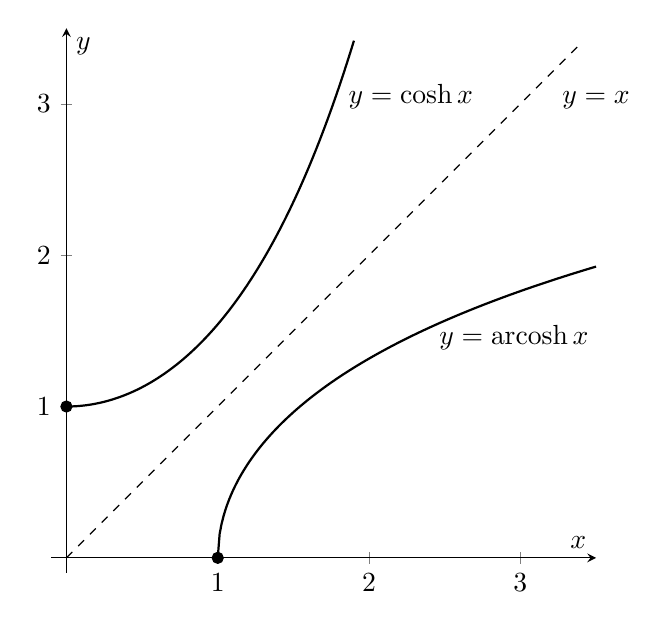
\begin{tikzpicture}
\begin{axis}[
width=8.5cm,
height=8.5cm,
axis lines=middle,
xmin=-0.1, xmax=3.5,
ymin=-0.1, ymax=3.5,
xlabel={$x$},
ylabel={$y$},
xtick={1,2,3},
ytick={1,2,3},
samples=200,
clip=false,
axis equal image
]
\addplot[thick,domain=0:1.9] {(exp(x)+exp(-x))/2};
\addplot[thick,domain=1:3.5] {ln(x + sqrt(x^2 - 1))};
\addplot[dashed,domain=0:3.4] {x};
\addplot[only marks,mark=*] coordinates {(0,1) (1,0)};
\node[above right] at (axis cs:1.8,2.9) {$y=\cosh x$};
\node[below right] at (axis cs:2.4,1.6) {$y=\operatorname{arcosh}x$};
\node[above] at (axis cs:3.5,2.9) {$y=x$};
\end{axis}
\end{tikzpicture}

because:

For \(y=\cosh x\), when \(x=0\),
\[
y=\cosh 0=1
\]
so the curve starts at \((0,1)\).

Its gradient is
\[
\frac{\mathrm{d}y}{\mathrm{d}x}=\sinh x
\]
Hence at \(x=0\),
\[
\frac{\mathrm{d}y}{\mathrm{d}x}=\sinh 0=0
\]
so the tangent there is horizontal.

For \(x\ge 0\), \(y=\cosh x\) increases and is convex.

Now \(y=\operatorname{arcosh}x\) is the inverse of \(y=\cosh x\) for \(x\ge 0\), so its graph is the reflection of \(y=\cosh x\) in the line \(y=x\). Therefore it starts at \((1,0)\) and increases for \(x\ge 1\).

So the line of symmetry is
\[
y=x
\]


Therefore the gradient at \(x=0\) is \(0\), and the line of symmetry is \(y=x\).

\item
\[
\int_0^k \cosh x\,\mathrm{d}x=[\sinh x]_0^k
\]
So
\[
\int_0^k \cosh x\,\mathrm{d}x=\sinh k-\sinh 0=\sinh k
\]

Hence
\[
\int_0^k \cosh x\,\mathrm{d}x=\sinh k
\]

\item Since \(y=\operatorname{arcosh}x\) is the inverse of \(y=\cosh x\), the two graphs are reflections of each other in the line \(y=x\).

Therefore, the area under \(y=\cosh x\) from \(x=0\) to \(x=k\) and the area under \(y=\operatorname{arcosh}x\) from \(x=1\) to \(x=\cosh k\) together make the rectangle of width \(k\) and height \(\cosh k\). So
\[
\int_0^k \cosh x\,\mathrm{d}x+\int_1^{\cosh k}\operatorname{arcosh}x\,\mathrm{d}x=k\cosh k
\]

From part (ii),
\[
\int_0^k \cosh x\,\mathrm{d}x=\sinh k
\]
Substituting gives
\[
\sinh k+\int_1^{\cosh k}\operatorname{arcosh}x\,\mathrm{d}x=k\cosh k
\]
Hence
\[
\int_1^{\cosh k}\operatorname{arcosh}x\,\mathrm{d}x=k\cosh k-\sinh k
\]

Therefore
\[
\int_1^{\cosh k}\operatorname{arcosh}x\,\mathrm{d}x=k\cosh k-\sinh k
\]
\end{enumerate}
\end{tcolorbox}


\end{enumerate}
\end{document}
